\newpage
\section{Problem 5.7}
\subsection{重要参数}

\[g(x)=f'(x)=9-\dfrac{4}{x-7}\]
\[G(x)=g'(x)=\dfrac{4}{(x-7)^2}\]

其迭代公式为:
\[x^{(k+1)}=x^{(k)}-\dfrac{1}{4}(x^{(k)}-7)(9x^{(k)}-67)\]


\subsection{算法伪代码}
\begin{algorithm}[h]  
\caption{Newton method for problem(5.7)}  
\begin{algorithmic}[1]  
\STATE Given $x^{(0)}$ and compute $g(x)=f'(x)$
\STATE Compute $G(x)=g'(x)$
\STATE Set $g^{(0)}=g(x^{(0)}),k=0$
\WHILE {$|g^{(k)}|>\epsilon$}
\STATE Set $s^{(k)}=-g^{(k)}/G^{(k)}$
\STATE Set $x^{(k+1)}=x^{(k)}+s^{(k)}$
\STATE Set k=k+1
\ENDWHILE
\end{algorithmic}  
\end{algorithm}  



\subsection{计算结果展示}
% Table generated by Excel2LaTeX from sheet 'Sheet1'
\begin{table}[htbp]
  \centering
  \caption{迭代5次过程}
    \begin{tabular}{clllll}
\toprule
  $x^{(0)}$&7.4  & 7.2  & 7.01 &7.80  & 7.88 \\
	\midrule
   $x^{(1)}$& 7.44  & 7.31  & 7.019775 & 7.16  & 7.0176 \\
    $x^{(2)}$&7.4444 & 7.403775 & 7.038670136 & 7.2624 & 7.03450304 \\
    $x^{(3)}$&7.44444444 & 7.440722936 & 7.073975668 & 7.36987904 & 7.066327546 \\
   $ x^{(4)}$&7.444444444 & 7.444413283 & 7.135638438 & 7.431934445 & 7.122756569 \\
    $x^{(5)}$&7.444444444 & 7.444444442 & 7.229881858 & 7.444092319 & 7.211607493 \\
	\midrule
    $f(x^{(5)})$&70.24372086 & 70.24372086 & 70.94969577 & 70.24372212 & 71.11655611 \\
	\bottomrule
    \end{tabular}%
  \label{tab:addlabel}%
\end{table}%

% Table generated by Excel2LaTeX from sheet 'Sheet1'
\begin{table}[htbp]
  \centering
  \caption{大范围迭代结果}
    \begin{tabular}{|c|c|c|c|}
    \hline
    初始点   & 迭代终止点 & 初始点   & 迭代终止点 \\
    \hline
    5     & -Inf  & 9     & -Inf \\
    \hline
    5.25  & -Inf  & 9.25  & -Inf \\
    \hline
    5.5   & -Inf  & 9.5   & -Inf \\
    \hline
    5.75  & -Inf  & 9.75  & -Inf \\
    \hline
    6     & -Inf  & 10    & -Inf \\
    \hline
    6.25  & -Inf  & 10.25 & -Inf \\
    \hline
    6.5   & -Inf  & 10.5  & -Inf \\
    \hline
    6.75  & -Inf  & 10.75 & -Inf \\
    \hline
    7     & 7     & 11    & -Inf \\
    \hline
    7.25  & 7.44444444444445 & 11.25 & -Inf \\
    \hline
    7.5   & 7.44444444444445 & 11.5  & -Inf \\
    \hline
    7.75  & 7.44444444444445 & 11.75 & -Inf \\
    \hline
    8     & -Inf  & 12    & -Inf \\
    \hline
    8.25  & -Inf  & 12.25 & -Inf \\
    \hline
    8.5   & -Inf  & 12.5  & -Inf \\
    \hline
    8.75  & -Inf  & 12.75 & -Inf \\
    \hline
    \end{tabular}%
  \label{tab:addlabel}%
\end{table}%


由MATLAB函数fminsearch求得最优解为:\[x^{\star}=7.444421386718750,\quad f(x^{\star})=70.243720870248540\]

\begin{figure}[H]
\centering
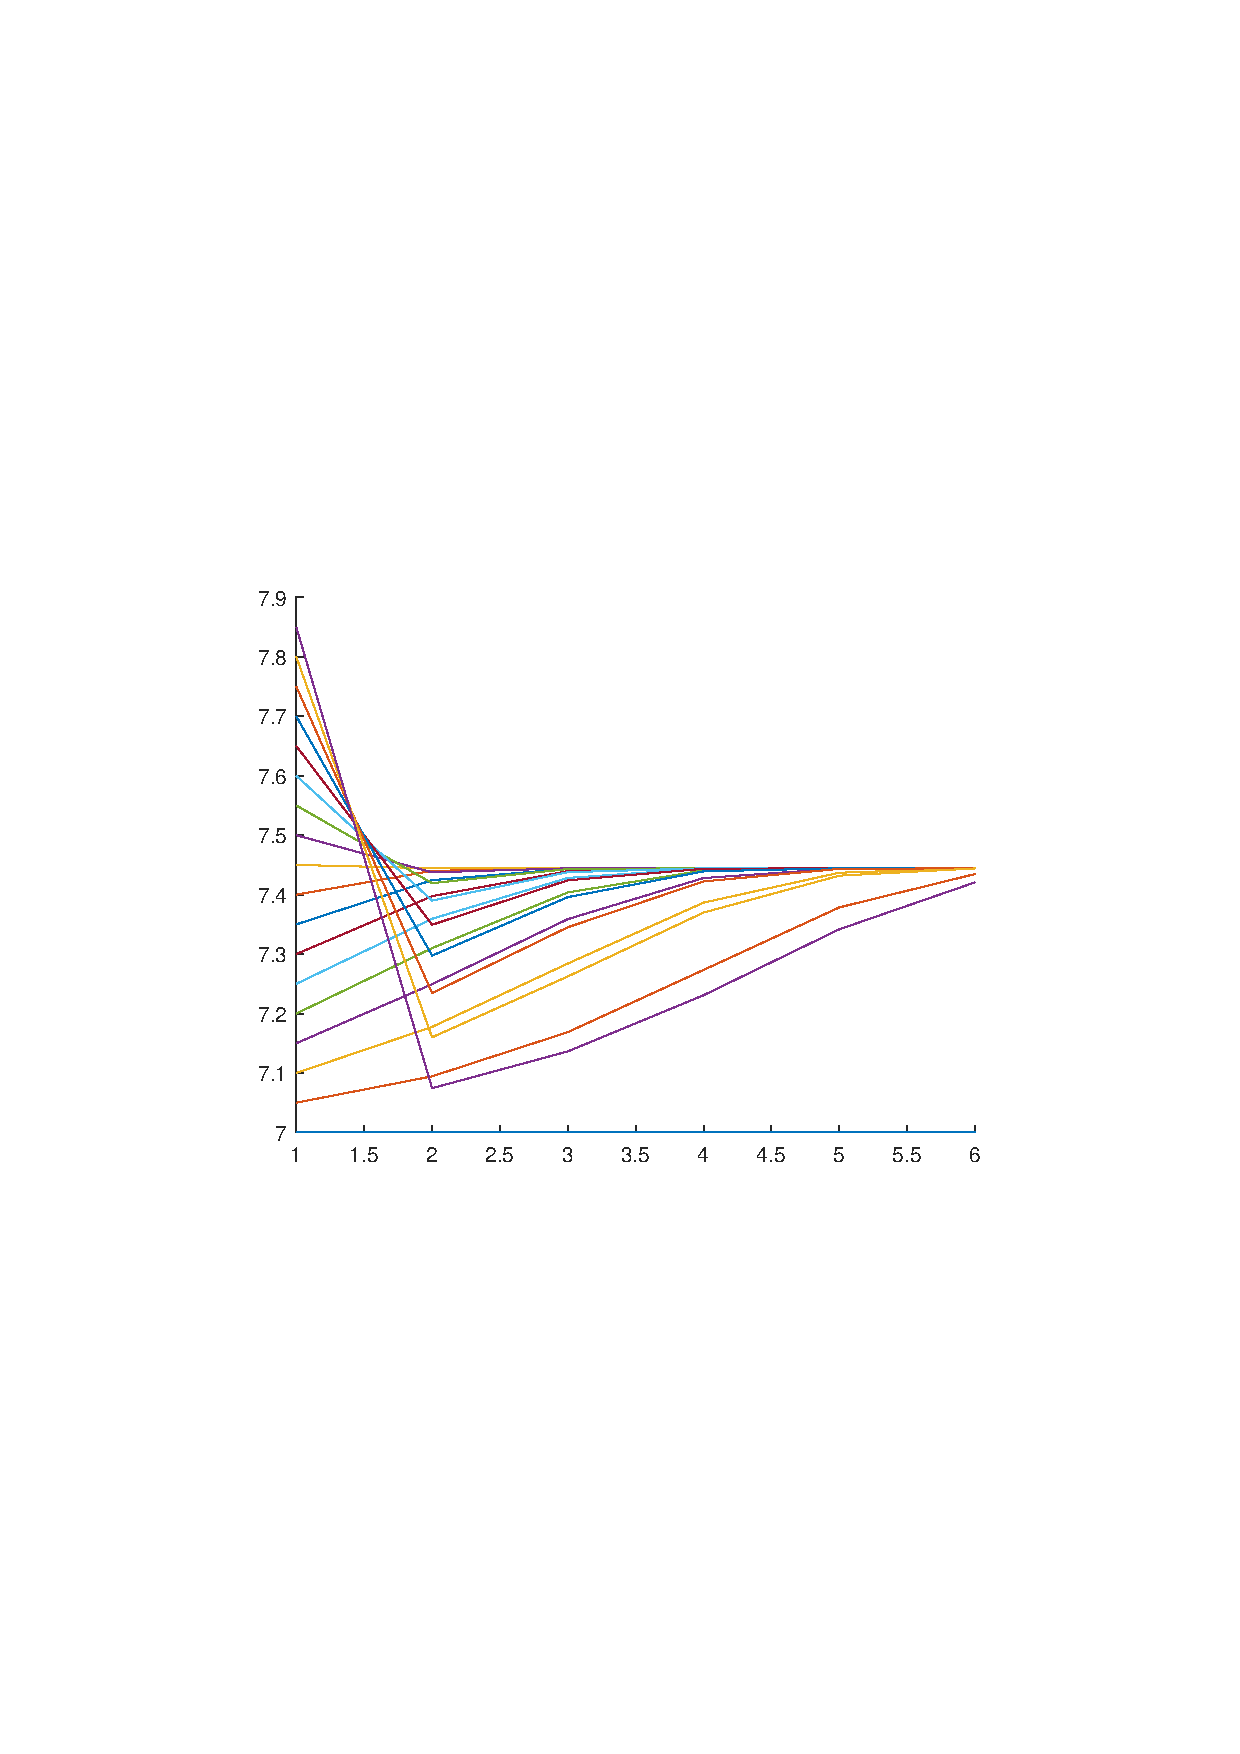
\includegraphics[width=10cm]{fig/2_1.pdf}
\end{figure}

\begin{figure}[H]
\centering
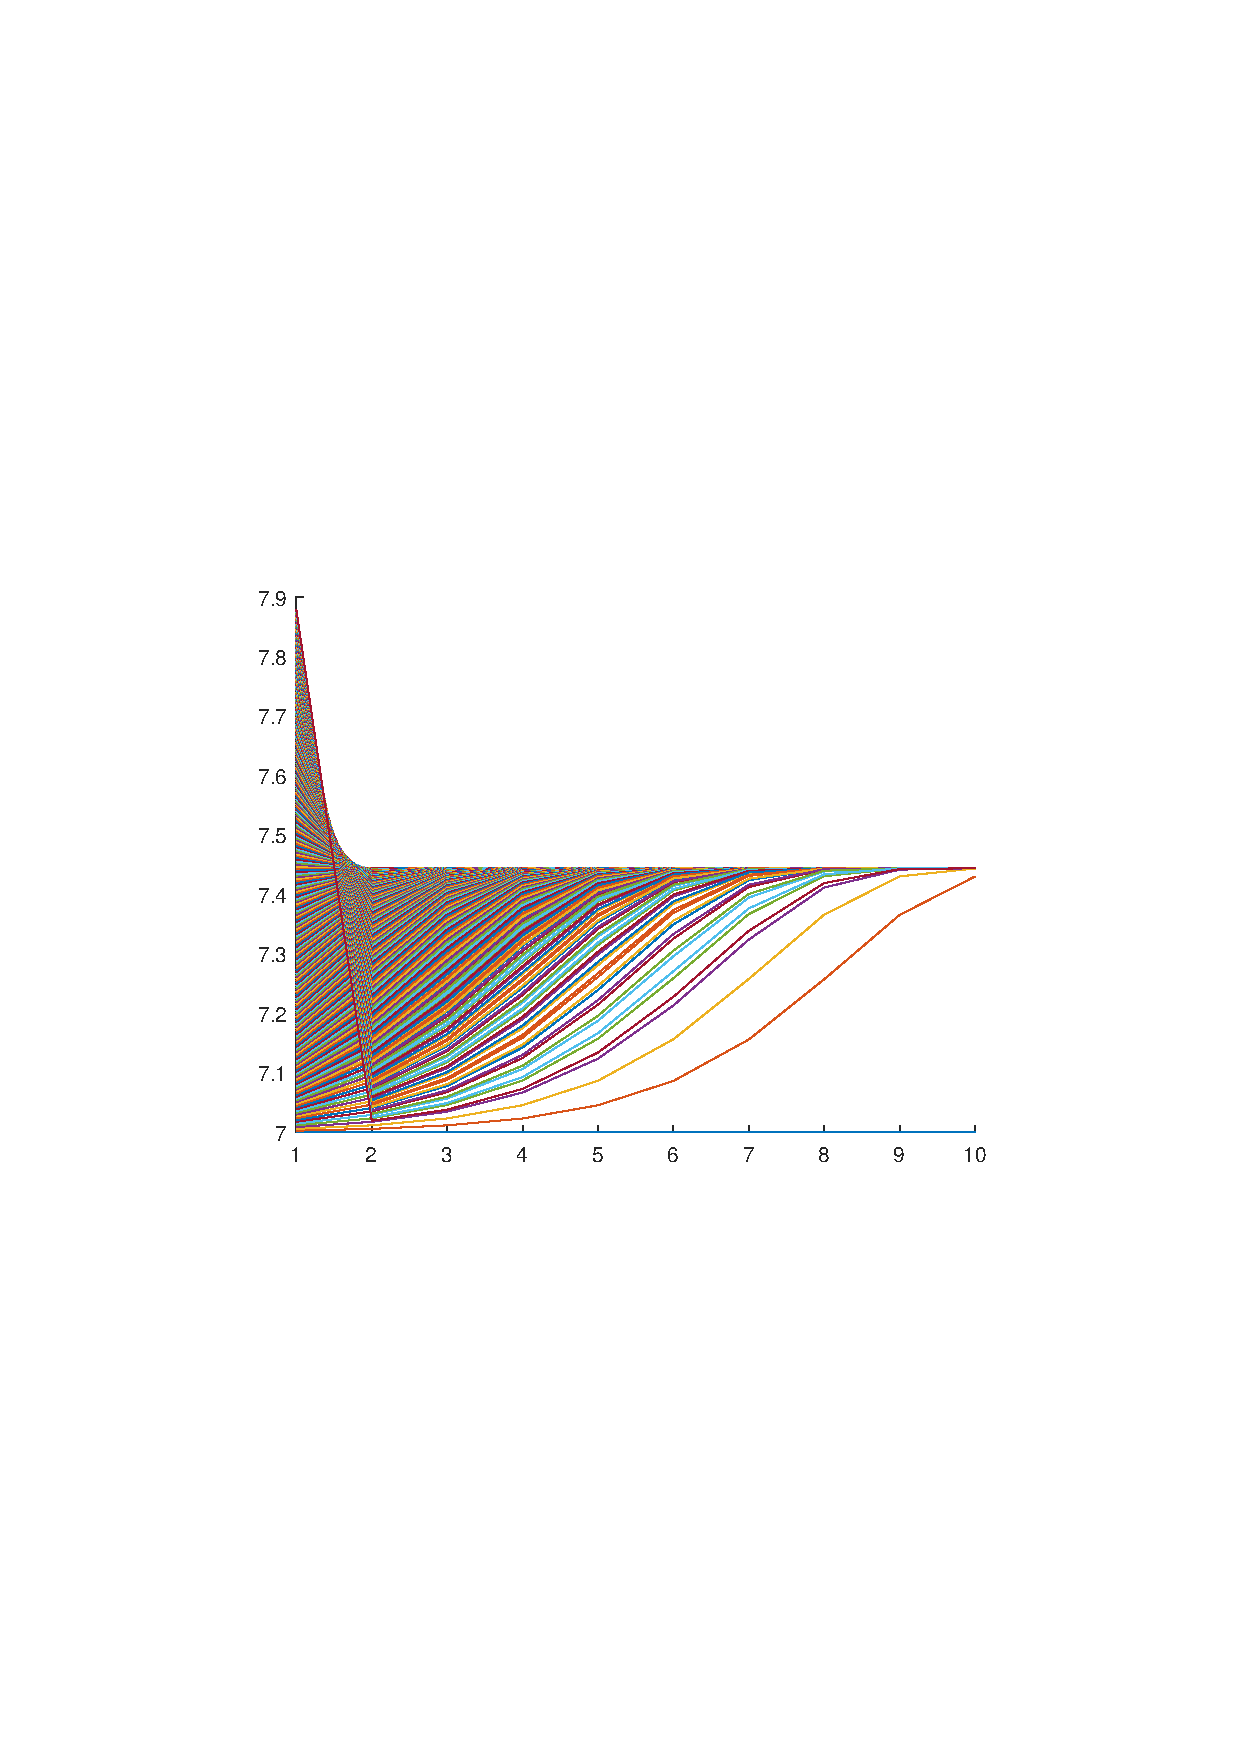
\includegraphics[width=10cm]{fig/2_2.pdf}
\end{figure}






